\section{Arquitetura Lógica do Sistema}

\begin{figure}
    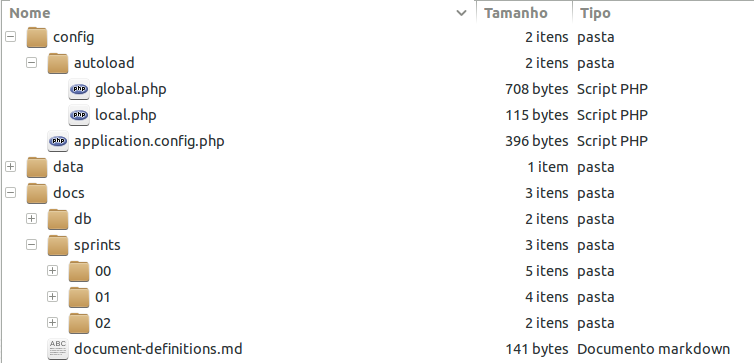
\includegraphics[scale=0.5]{img/arquitetura-pacotes-01.png}
    \caption{Parte 1}
\end{figure}

\subsection{Referente a figura Parte 1}

\paragraph{config/application.config.php}

Define quais módulos serão utilizados e quais bibliotecas externas devem
ser carregadas.

\paragraph{config/autoload/*}

Define variáveis globais, locais, parâmetros de conexão com banco de
dados.

\paragraph{docs/db/*}

Arquivos para criação do banco de dados e restrições ACL.

\paragraph{docs/sprints/*}

Arquivos e artefatos dos sprints numerados sequencialmente: 00, 01, 02,
\ldots{}

\begin{figure}
    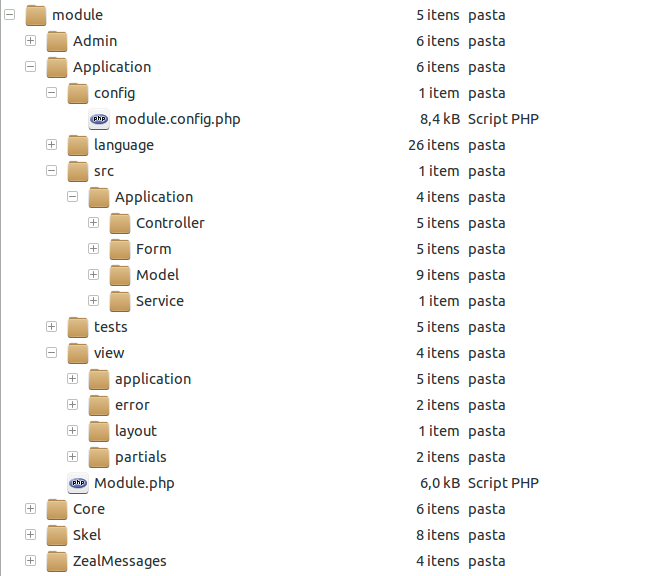
\includegraphics[scale=0.5]{img/arquitetura-pacotes-02.png}
    \caption{Parte 2}
\end{figure}

\subsection{Referente a figura Parte 2}

\paragraph{modules/*}

Cada diretório representa um módulo. Módulos no Zend2 foram feitos para
serem genéricos e poderosos onde podemos criar nossas próprias
funcionalidades e \emph{plugins}.

Por exemplo, \textbf{Admin} e \textbf{Application} são módulos MVC.
\textbf{ZealMessages} é um módulo para mostrar mensagens de uma
\emph{action} para outra na tela do usuário. No módulo \textbf{Core}
temos implementações iniciais de algumas classes e classes que vão ser
usadas por outros módulos MVC.

\paragraph{modules/Application/*}

Módulo MVC principal, com todos os componentes e interfaces de usuário
que interessam ao usuário comum.

\paragraph{modules/Application/config/module.config.php}

Responsável pelo mapeamento de rotas, mapeamentos dos
\emph{Controllers}, instanciação dos \emph{Models}, carregar arquivos
\emph{gettext} para a internacionalização (i18n).

\paragraph{modules/Application/language/*}

Contém os arquivos \emph{.po} usados pelo \emph{gettext}.

\paragraph{modules/Application/src/Application/*}

Possui a estrutura:

\begin{itemize}
\item
  \textbf{Controller}: trata da regra de negócios.
\item
  \textbf{Form}: classes responsáveis pelos formulários e filtros de
  validação.
\item
  \textbf{Model}: classes modelo e classes de acesso ao banco.
\item
  \textbf{Service}: serviços, como autenticação.
\end{itemize}
\paragraph{modules/Application/tests/*}

Testes unitários do sistema.

\paragraph{modules/Application/view/*}

Único local que código \emph{PHP} é misturado com \emph{HTML}. Sua
estrutura:

\begin{itemize}
\item
  \textbf{application}: arquivos \emph{.phtml} referentes aos
  \emph{controllers/actions} do módulo \emph{application}.
\item
  \textbf{error}: \emph{layout} para páginas de erro, podemos criar
  layouts para erro \emph{404 (Not Found)}, etc.
\item
  \textbf{layout}: \emph{layout} que faz \emph{wrapper} (envolve) todas
  as páginas, contém código comum a todas as páginas e inclui todas as
  outras.
\item
  \textbf{partials}: trechos de código que se repetem, ou trechos não
  acoplados que são separados para deixar código mais limpo e de fácil
  manutenção.
\end{itemize}
\begin{figure}
    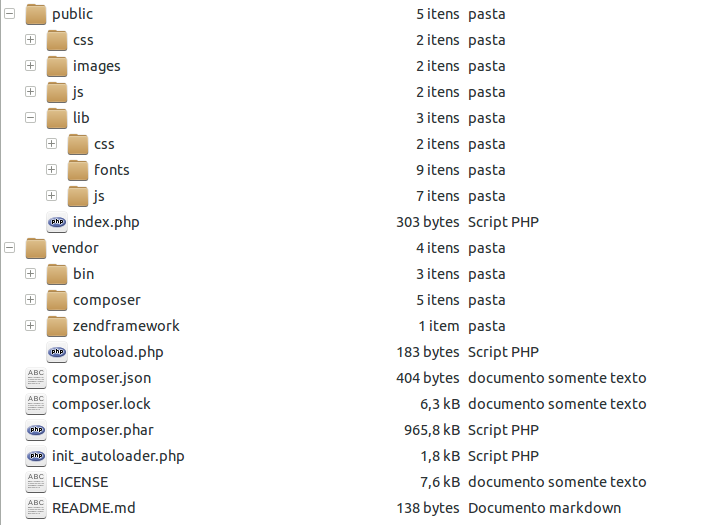
\includegraphics[scale=0.5]{img/arquitetura-pacotes-03.png}
    \caption{Parte 3}
\end{figure}

\subsection{Referente a figura Parte 3}

\paragraph{public/*}

Contém todos os arquivos públicos. Sua estrutura:

\begin{itemize}
\item
  \textbf{css}: folhas de estilo.
\item
  \textbf{js}: arquivos javascript.
\item
  \textbf{images}: arquivos de imagens.
\item
  \textbf{lib}: bibliotecas externas.
  \begin{itemize}
  \item
    \textbf{css}: folhas de estilo das bibliotecas externas.
  \item
    \textbf{js}: arquivos javascript.
  \item
    \textbf{fonts}: web fonts.
  \end{itemize}
\end{itemize}
\paragraph{public/index.php}

Único arquivo php público responsável por fazer o Bootstrap (arranque)
do sistema.
